%%%%%%%%%%%%%%%%%%%%%%%%%%%%%%%%%%%%%%%%%
% Simple Sectioned Essay Template
% LaTeX Template
%
% This template has been downloaded from:
% http://www.latextemplates.com
%
% Note:
% The \lipsum[#] commands throughout this template generate dummy text
% to fill the template out. These commands should all be removed when 
% writing essay content.
%
%%%%%%%%%%%%%%%%%%%%%%%%%%%%%%%%%%%%%%%%%

%----------------------------------------------------------------------------------------
%	PACKAGES AND OTHER DOCUMENT CONFIGURATIONS
%----------------------------------------------------------------------------------------

\documentclass[12pt]{article} % Default font size is 12pt, it can be changed here

\usepackage{geometry} % Required to change the page size to A4
\geometry{a4paper} % Set the page size to be A4 as opposed to the default US Letter

\usepackage{graphicx} % Required for including pictures

\usepackage{float} % Allows putting an [H] in \begin{figure} to specify the exact location of the figure
\usepackage{wrapfig} % Allows in-line images such as the example fish picture

\usepackage{lipsum} % Used for inserting dummy 'Lorem ipsum' text into the template

\usepackage{color}
\usepackage{mathtools}
\usepackage{graphicx}
\usepackage{hyperref}
\hypersetup{
colorlinks=true,
linkcolor=blue,
urlcolor=blue
}
\usepackage{braket}
\usepackage{cancel}
\usepackage{acronym}
\acrodef{stem}[STEM]{Scanning Transmission Electron Microscopy}
\acrodef{tem}[STEM]{Transmission Electron Microscope}
\acrodef{cemn}[CEMN]{Center for Electron Microscopy and Nanofabrication}
\acrodef{edx}[EDX]{Energy-dispersive X-ray spectroscopy}
% http://staff.science.uva.nl/~polko/HOWTO/LATEX/acronym.html 

\usepackage{epstopdf}
\epstopdfDeclareGraphicsRule{.tif}{png}{.png}{convert #1 \OutputFile}
\AppendGraphicsExtensions{.tif}

%\setlength\parindent{0pt} % Uncomment to remove all indentation from paragraphs

\graphicspath{Data/} % Specifies the directory where pictures are stored

\title{TEM Report 2}
\author{Bret Comnes}
\date{\today}


\begin{document}
\maketitle

\section{Introduction} % Major section

This report will cover some basics concepts relating to \ac{stem} and \ac{edx}, as well as some simple analysis of data taken a student lab session at the \ac{cemn} at Portland State University on \date{May 16, 2014}.  Bright field \ac{stem} images, \ac{edx} data and point spectrum of the inspected sample are included.  The data was collected using a FEI Technai \ac{tem} and the accompanying AZtec EDS acquisition and analysis tool.

Spectrum analysis is performed using last available freely distributed version of Fityk\cite{ft}: v.0.9.8.  Additional work was performed to build newer versions of Fityk from source for additional analysis  and add it to the Homebrew\cite{HB} package manager for future convenience.


\section{\ac{stem} Fundamentals} % (fold)
\label{sec:stem}

Stem stuff

% section stem (end)


\section{\ac{edx} fundamentals} % (fold)
\label{sec:edx}

edx stuff

% section acedx_fundamentals (end)

\section{Data Analysis} % (fold)
\label{sec:data_analysis}

We collected bright field TEM images of a Iron Oxide ($Fe_3O_4$) particles coated with Silicon dioxide ($SiO_2$).  Additionally, we collected \ac{edx} spectrum information and mapped the location of these different elements using the AZtec software.  The data was explored in a limited manner use the Fityk software.  Unfortunately the \ac{stem} images were lost in the process of exporting data and cannot be included.

\subsection{TEM imaging} % (fold)
\label{sub:tem_imaging}

Bright field images of Iron Oxide particles coated with Silicon dioxide.

\begin{figure}[htbp]
  \centering
  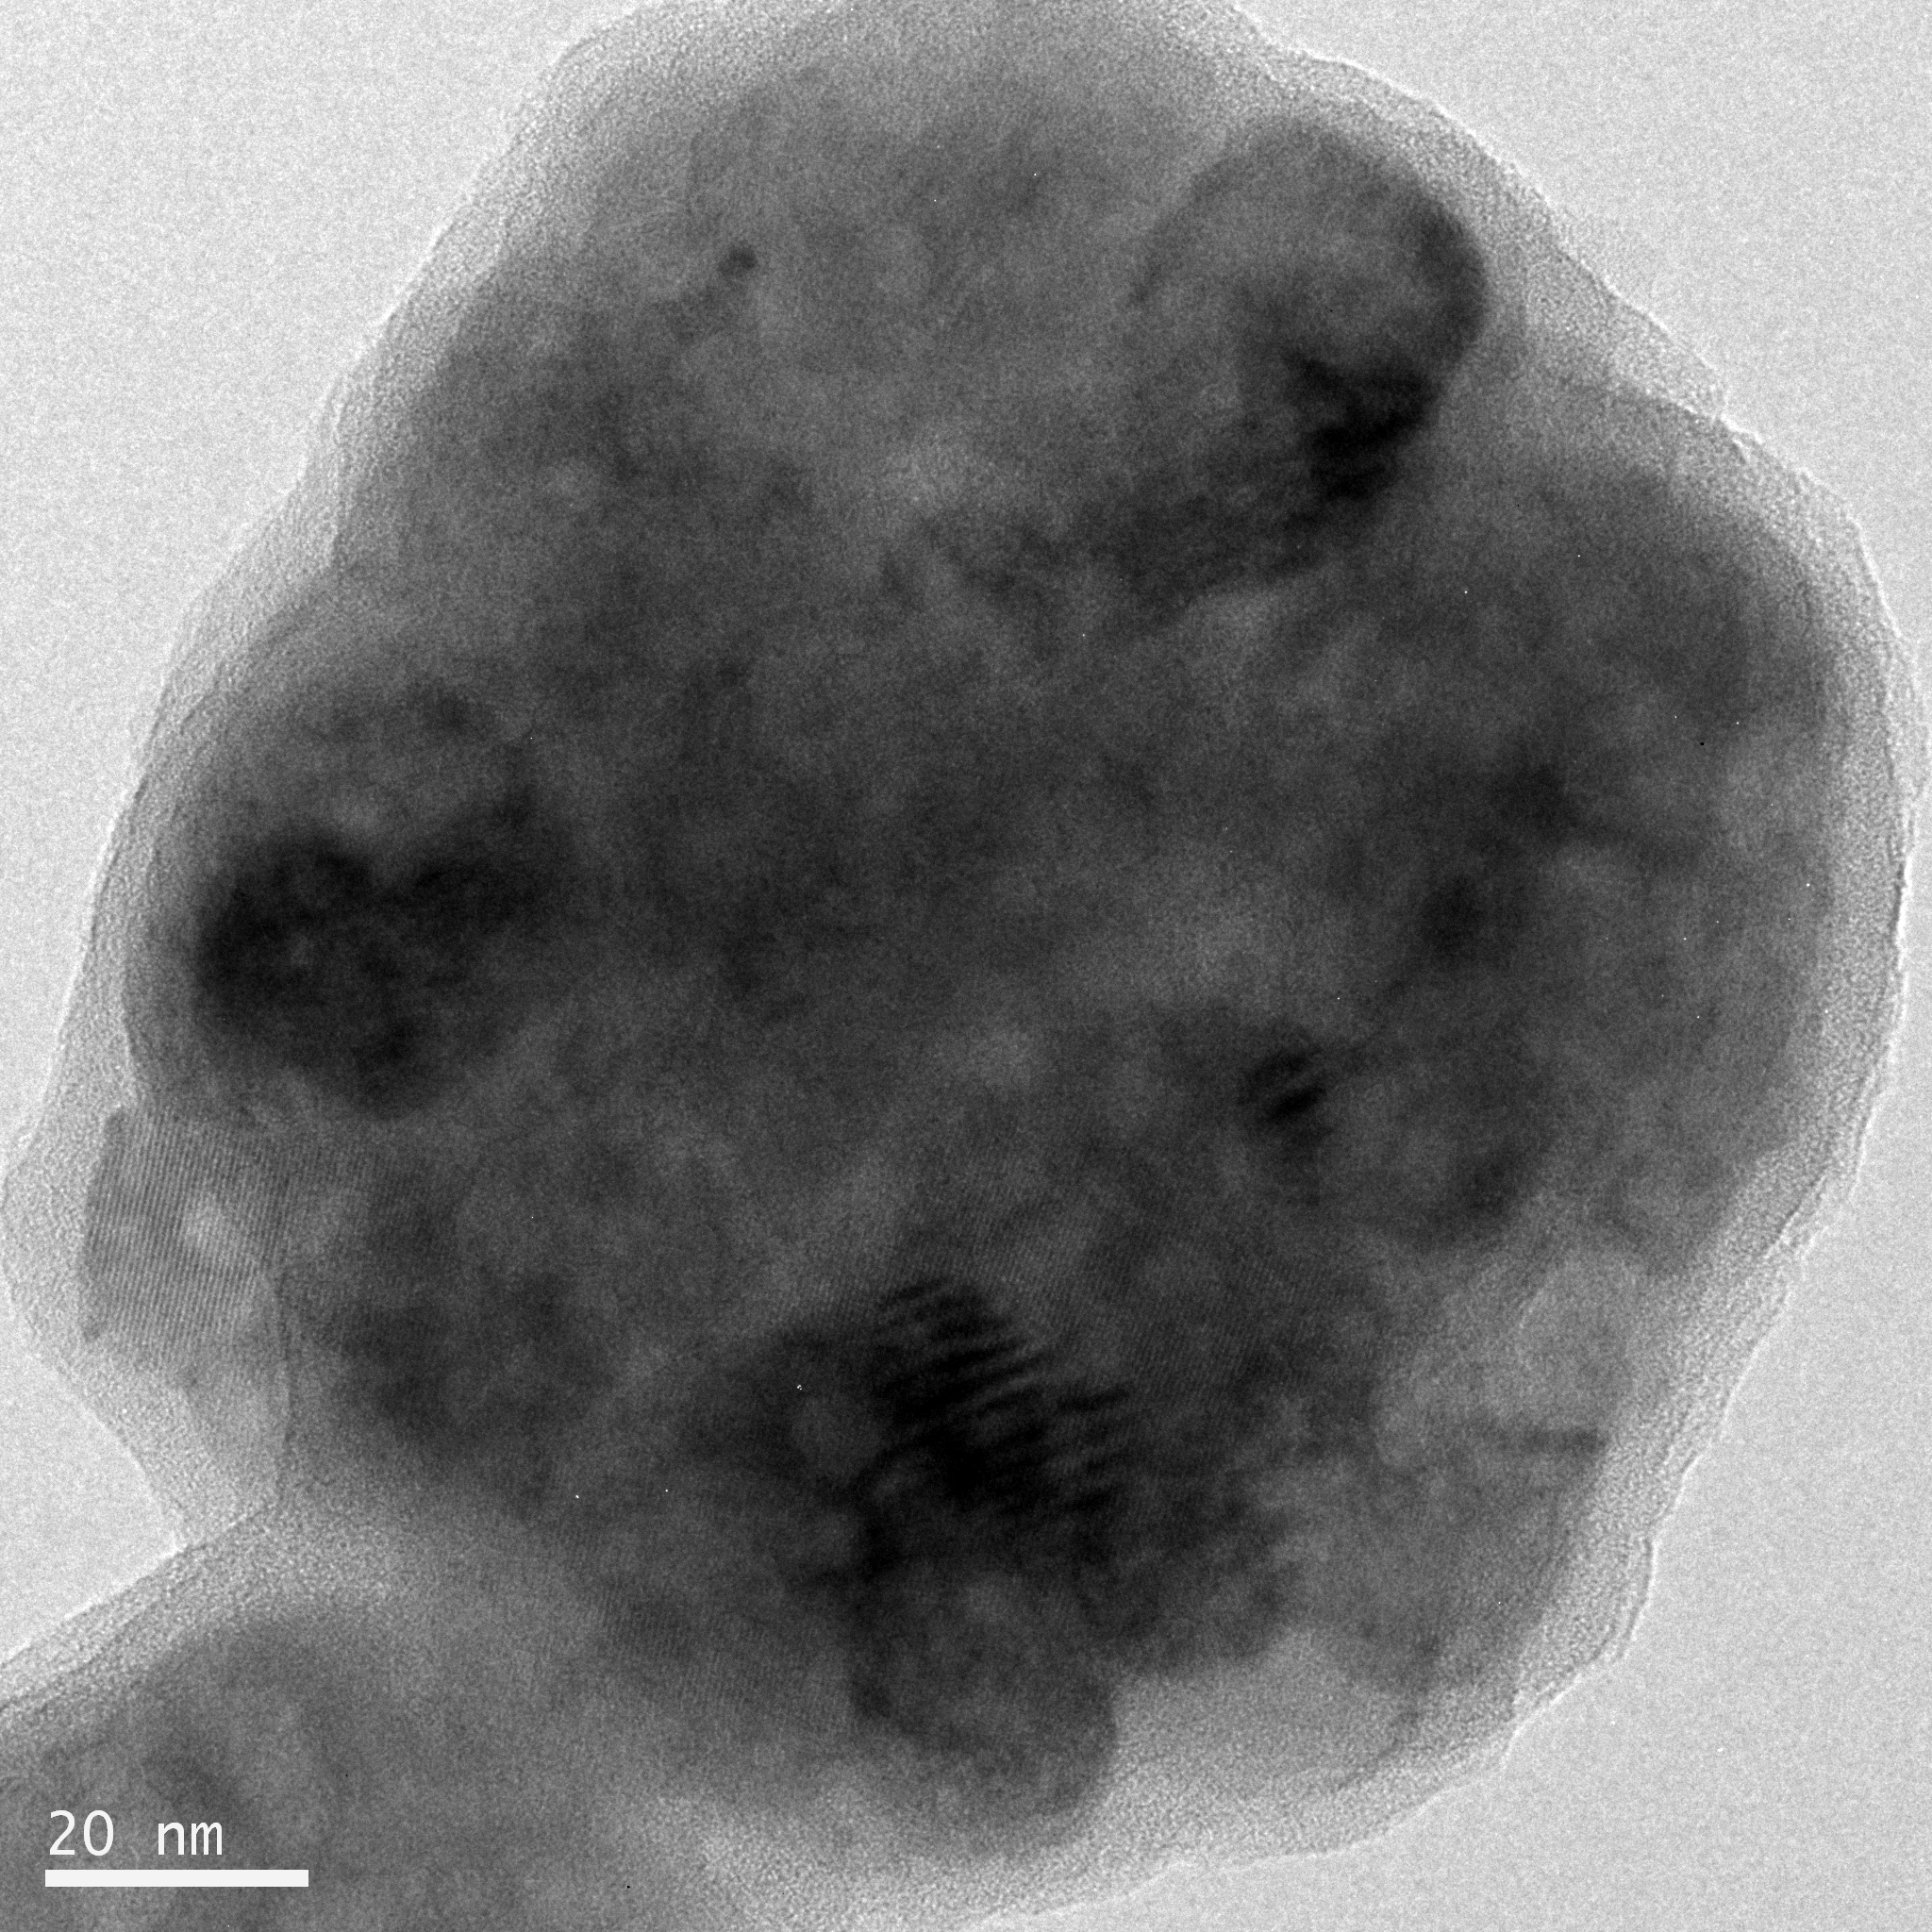
\includegraphics[width=0.95\textwidth]{Data/Fe3O4-SiO2-0001.eps}
  \caption{caption}
  \label{fig:label}
\end{figure}

% subsection tem_imaging (end)

\subsection{EDX Spectroscopy} % (fold)
\label{sub:edx_spectroscopy}

% subsection edx_spectroscopy (end)

\subsection{EDS Maps} % (fold)
\label{sub:eds_maps}

% subsection eds_maps (end)

% section data_analysis (end)

\section{Conclusion} % Major section


Conclusion statements


\bibliography{main} 
\bibliographystyle{plain} \nocite{*}

\end{document}